
\subsection{On récapitule}
La Figure~\ref{fig:composants} illustre quelques exemples des trois types de composants que l'on trouve sur un réseau.

\begin{figure}[h!t]
\centering
  \begin{subfigure}{.49\textwidth}
    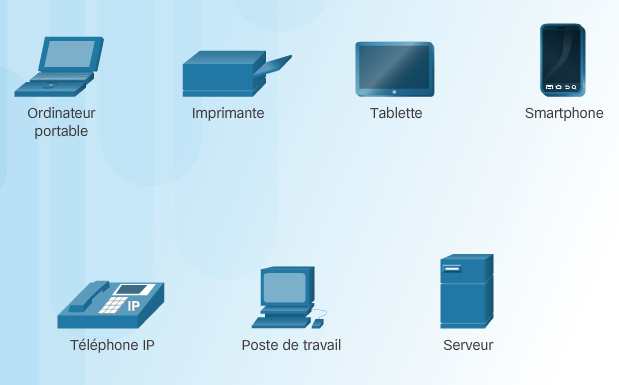
\includegraphics[width=\linewidth]{images/materiel/terminaux}
    \caption{Exemples de périphériques finaux}
  \end{subfigure}
  \begin{subfigure}{.49\textwidth}
    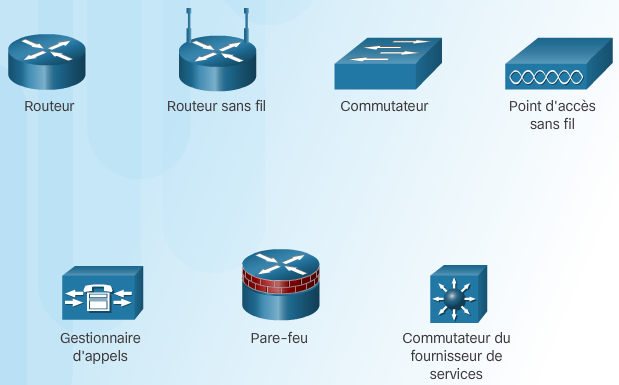
\includegraphics[width=\linewidth]{images/materiel/intermediaires}
    \caption{Exemples de périphériques intermédiaries}
  \end{subfigure}

  \begin{subfigure}{.98\textwidth}
    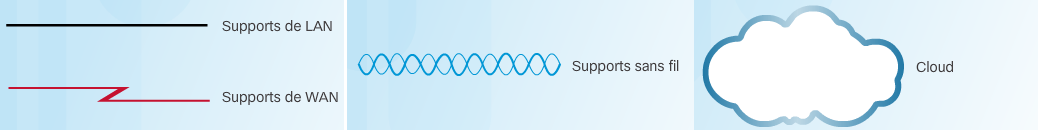
\includegraphics[width=\linewidth]{images/materiel/supports}
    \caption{Exemples de supports de communication}
  \end{subfigure}
  \caption{Différents composants d'un réseau. \textit{Source : Cours NetAcad 1.2.2.1}}
  \label{fig:composants}
\end{figure}

Le Tableau~\ref{tab:materiel} (inspiré du site OpenClassRooms) regroupe les différents materiels abordés et leur fonctions principales.

\begin{table}[h!t]
\centering
  \begin{tabular}{l|p{.6\textwidth}}
  \textbf{Matériel} & \textbf{Fontion} \\\hline
  Carte réseau & La carte réseau est le matériel de base indispensable, qui traite tout au sujet de la communication dans le monde du réseau.\\\hline

Concentrateur (hub) & Le concentrateur permet de relier plusieurs ordinateurs entre eux, mais on lui reproche le manque de confidentialité. On peut le voir comme une simple «multi-prise» Ethernet. \\\hline

Commutateur (switch) & Le commutateur fonctionne comme le concentrateur, sauf qu'il transmet des données aux destinataires en se basant sur leurs adresses MAC (adresses physiques). Chaque machine reçoit seulement ce qui lui est adressé.\\\hline

Routeur & Le routeur permet d'assurer la communication entre différents réseaux pouvant être fondamentalement différents (réseau local et Internet).\\\hline

Répéteur& Le répéteur reçoit des données par une interface de réception et les renvoie plus fort par l'interface d'émission. On parle aussi de relais en téléphonie et radiophonie.\\
\end{tabular}

  \caption{Récapitulatif des matériels abordés}
  \label{tab:materiel}
\end{table}
